% !TeX root = ../../../main.tex
\begin{ChFiveUncaptionedFigure}
\begin{ChFiveFloatBody}
  % float page; will try to use its own page
  \centering
   %%%%%%%%%%%%%%%%%%%%%%%%%%%%%% 
    \begin{tcolorbox}[colback=white,colframe=black!30,boxrule=0.6pt,left=2mm,right=2mm,top=2mm,bottom=2mm,width=\linewidth]
    \footnotesize \textbf{Excerpt from \cite{abu2023rare}:}
    \begin{quote}\footnotesize
    A 57-year-old man recently diagnosed with lepromatous leprosy was confirmed with skin biopsy and had been on treatment (rifampicin/clofazimine/dapsone) for 2 months before admission; he was presented to the hospital with complaints of abdominal distension, constipation, vomiting, and a 10-kg weight loss. On examination, the patient was vitally stable. He had evidence of peripheral lymphadenopathy with a distended abdomen and a positive shifting dullness. A computed tomography scan of his abdomen showed mural thickening of the terminal ileum with significantly enlarged mesenteric lymph nodes, mesenteric fat stranding, and intra-abdominal free fluid, suggesting abdominal granulomatous infection or neoplastic process.
    \dots 
    
    The patient was planned for consolidation by autologous bone marrow transplant. Unfortunately, with the recurrent bacteremia and sepsis that accompanied the patient’s course due to his immunocompromised state, he was re-admitted to the medical ICU for severe sepsis and multiorgan failure and passed away around 6 months after his initial diagnosis with NHL, despite maintaining a remission status.
    \end{quote}
    \end{tcolorbox}
    %\vspace{2pt}
    %%%%%%%%%%%%%%%%%%%%%%%%%%%%%% 
  % Row 1
  \begin{minipage}[t]{0.45\linewidth}\centering
    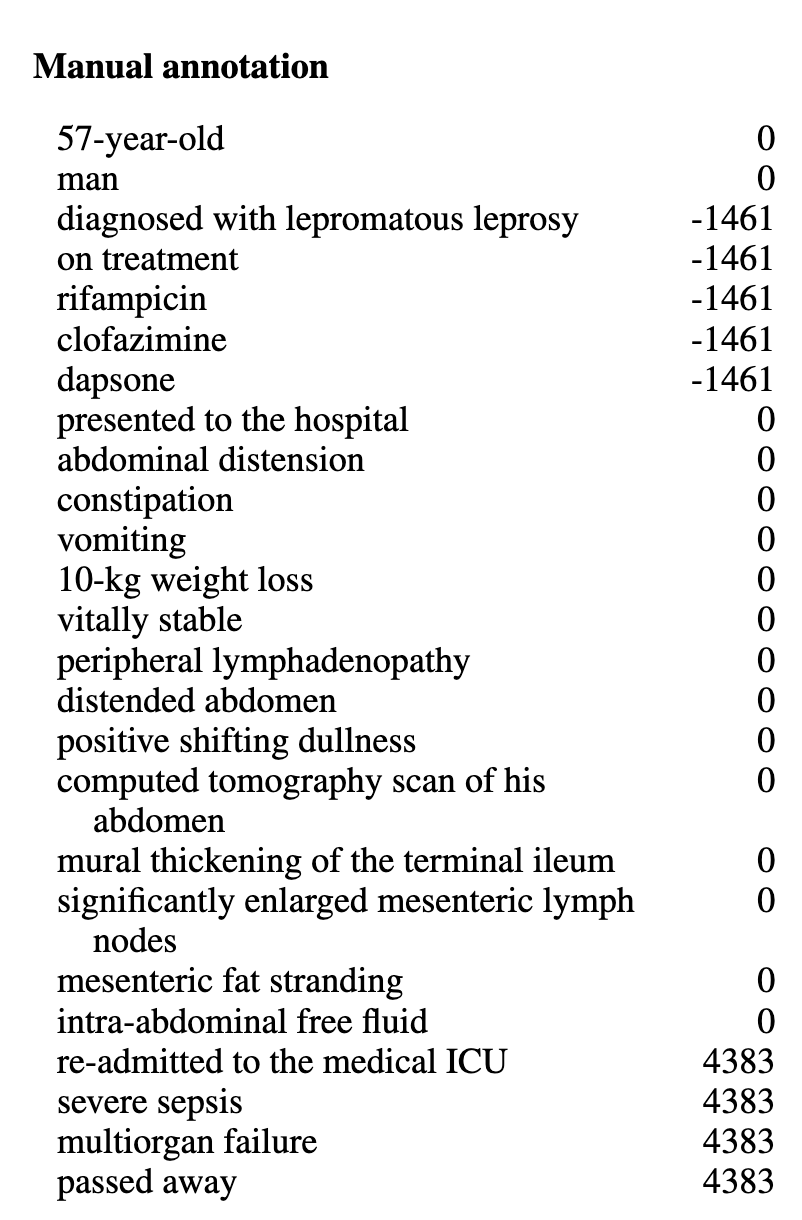
\includegraphics[width=0.9\linewidth]{Appendices/appendix-ch05/images/Scientific_data/Supplementary/example_TTS_for_paper/manual.png}
    %\caption{...}\label{fig:a}
  \end{minipage}\hfill
  \begin{minipage}[t]{0.45\linewidth}\centering
    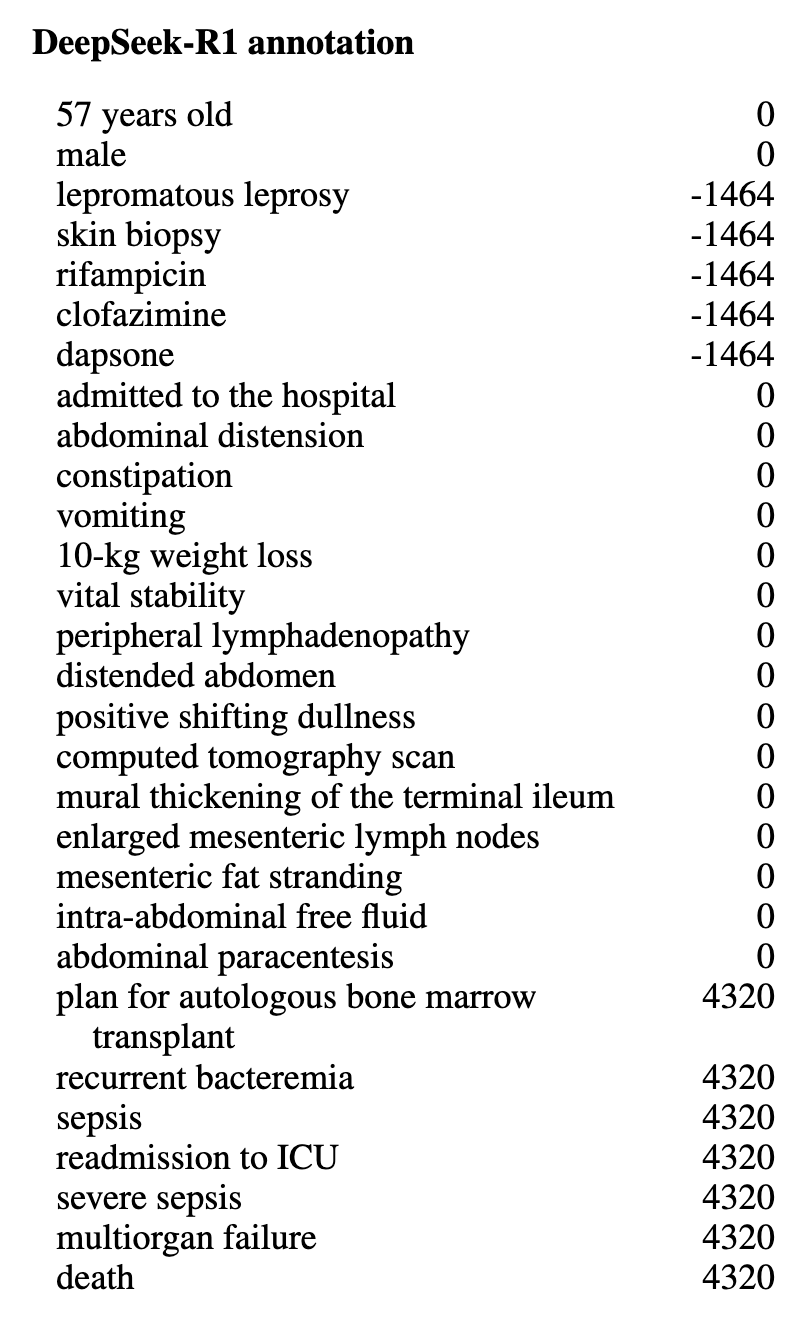
\includegraphics[width=0.9\linewidth]{Appendices/appendix-ch05/images/Scientific_data/Supplementary/example_TTS_for_paper/DeepSeekR1.png}
    %\caption{...}\label{fig:b}
  \end{minipage}

  %\vspace{6pt}

  % Row 2
  \begin{minipage}[t]{0.45\linewidth}\centering
    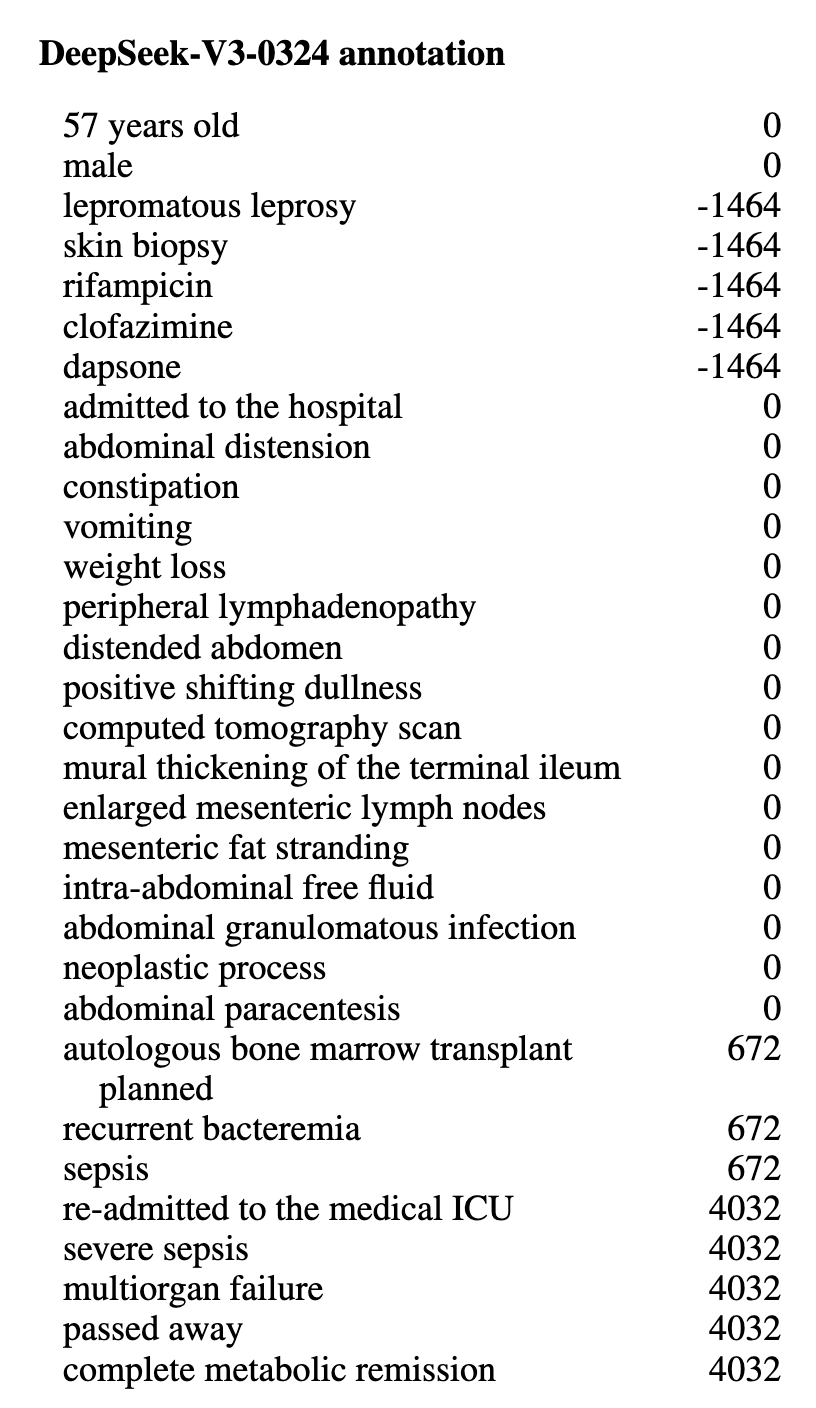
\includegraphics[width=0.9\linewidth]{Appendices/appendix-ch05/images/Scientific_data/Supplementary/example_TTS_for_paper/DeepSeekV3.png}
    %\caption{...}\label{fig:c}
  \end{minipage}\hfill
  \begin{minipage}[t]{0.45\linewidth}\centering
    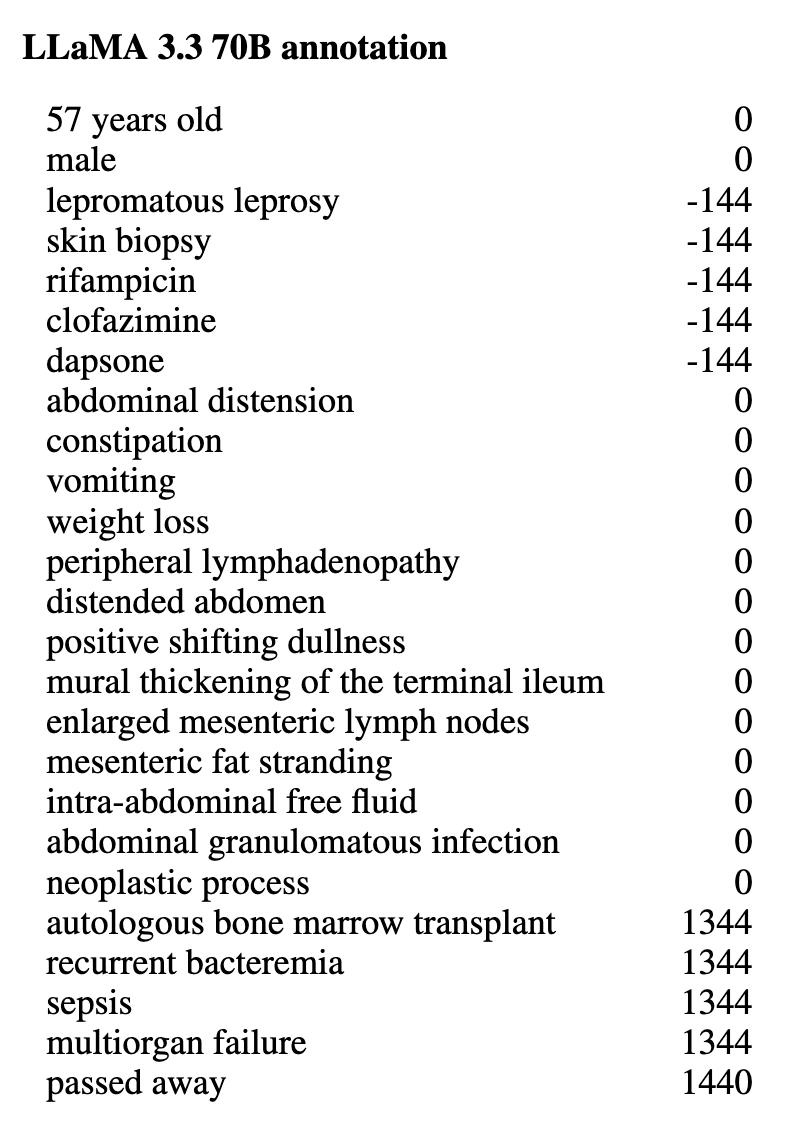
\includegraphics[width=0.9\linewidth]{Appendices/appendix-ch05/images/Scientific_data/Supplementary/example_TTS_for_paper/L3370B.png}
    %\caption{...}\label{fig:d}
  \end{minipage}
  %\caption{Overall caption for panels (a)–(d).}\label{fig:eight}

\end{ChFiveFloatBody}
\end{ChFiveUncaptionedFigure}